\documentclass[letter,10pt]{article}
\usepackage[utf8]{inputenc}
\usepackage{graphicx}
\usepackage{natbib}
\usepackage{hyperref}
\usepackage{courier}
\usepackage[margin=0.75in]{geometry}
\usepackage[table,svgnames]{xcolor}
\usepackage{multirow}
\usepackage{tabu}
\usepackage{float}
\usepackage{listings}
\usepackage{xspace} 
\bibliographystyle{unsrtnat}
\definecolor{HeaderColor}{rgb}{0.8, 0.8, 0.95}
\setlength{\parindent}{0pt}
\setlength{\parskip}{6pt}

\usepackage[T1]{fontenc}
\usepackage[utf8]{inputenc}
\usepackage{authblk}

\author[1,2]{Dimitri Yatsenko\thanks{dvyatsen@bcm.edu}}
\affil[1]{Department of Neuroscience, Baylor College of Medicine, Houston, Texas, USA}
\affil[2]{Vathes LLC, Houston, Texas, USA}

\renewcommand\Authands{ and }
\newcommand{\datajoint}{DataJoint\xspace}
\date{\today\\Revision 0.1}


\graphicspath{{./figures/}}

\lstset{
    backgroundcolor=\color{white},
    tabsize=4,
    basicstyle=\ttfamily,
    breaklines=true
    framextopmargin=50pt,
    aboveskip={0.5\baselineskip},
    columns=fixed,
    frame=single,
    showstringspaces=false,
    extendedchars=false,
    breaklines=true,
    numbers=none,
    showtabs=false,
    showspaces=false,
    showstringspaces=false,
    identifierstyle=\color[rgb]{0.0,0.2,0.0},
    keywordstyle=\bfseries\color[rgb]{0.2,0.2,0.6},
    commentstyle=\color[rgb]{0.4,0.6,0.6},
    stringstyle=\color[rgb]{0.6,0.0,0.2},
    numberstyle=\tiny\color[rgb]{0.6, 0.6, 0.6}}

\lstdefinelanguage{dj}{
  keywords={int, smallint, char, varchar, enum, unsigned, date, year, decimal},
  keywordstyle=\color{blue},
  keywords=[2]{boolean, string, number, objectid},
  keywordstyle=[2]\color{green}\bfseries,
  identifierstyle=\color{black},
  sensitive=true,
  morecomment=[l][\color{teal}\bfseries]{::},
  morecomment=[l][\color{gray}\itshape\small]{\#},
  stringstyle=\color{red},
  morestring=[b]',
  morestring=[b]"
}

\newfloat{lstfloat}{htbp}{lop}
\floatname{lstfloat}{Listing}

\title{\datajoint: A Simpler Relational Data Model}

\begin{document}

\maketitle
\begin{abstract}
A simplified and conceptually refined relational data model is proposed with a language for schema definition and data queries as well as a diagramming method for visualizing relationships among the data.  
Named \datajoint, the model adheres to the principle of \emph{entity normalization}, which requires that all data --- both stored and derived --- exist in the form of sets of entities belonging to well-defined entity classes.  
\datajoint's data query language is an algebra of five operators that provide equal capabilities to those of other relational query languages with greater clarity due to entity normalization. 
Practical implementations of \datajoint have been tested and adopted for scientific data pipelines by a number of leading neuroscience labs.  
With \datajoint, programmers interact with scientific data more fluently than with other data definition and query languages.
\end{abstract}
\tableofcontents 

\twocolumn

\section{Core Concepts}
\subsection{The Relational Data Model}
The relational data model \citep{codd_relational_1970} provides the most rigorous approach to structuring stored data as well as the most precise approach to querying stored data.  
Briefly, the relational data model is characterized by the principles of data representation, domain constraints, uniqueness constraints, referential constraints, and declarative queries as summarised in Table \ref{tab:core}.

\tabulinesep=6pt
\begin{table*}[ht]
\begin{tabu}{|X|}
\hline
{\bf Data representation.} Data are represented and manipulated in the form of \emph{relations}. 
A relation is a set (unordered collections) of \emph{tuples} of values for each of the respective named \emph{attributes} of the relation.
\emph{Base relations} represent stored data while \emph{derived relations} are formed from base relations as a result of data queries.
A collection of base relations with their attributes, domain constraints, uniqueness constraints, and referential constraints is called a \emph{schema}.

\\
{\bf Domain constraint.} Attribute values are drawn from corresponding attribute \emph{domains}, \emph{i.e.}\ predefined sets of values.
Attribute domains may not include other relations, ensuring that the relational model is essentially flat with no nesting data structures.

\\
{\bf Uniqueness constraints.} Tuples within relations are addressed by values of their attributes.
To identify and relate data elements, \emph{uniqueness constraints} on a subset of attributes may be imposed so that no two tuples can have the same values of these attributes.  The set of attributes with a uniqueness constraints are referred to as a \emph{key}. One in a relation key may be designated as the \emph{primary key} for the relation to serve for referencing elements in a relation.

\\
{\bf Referential constraints.} Associations among data are established by means of \emph{referential constraints} in the form of \emph{foreign keys}. 
Referential constraints prohibit tuples in one relation that lack tuples with matching values in the referenced relation. 

\\
{\bf Declarative queries.} \emph{Queries} produce derived relations from base relations and retrieve the result.  
\emph{Query expressions} provide declarative specifications for retrieved data rather than procedural specifications typical of other data models. 
Formal languages for query expressions include \emph{relational algebra} and \emph{relational calculus}.  
\\
\hline
\end{tabu}
\caption{Core principles of the relational data model.}
\label{tab:core}
\end{table*}

Popular implementations of the relational data model rely on the Structured Query Language (SQL) for schema definition, data manipulation, and data queries.
SQL so thoroughly dominates in the space of relational databases that it has become nearly synonymous with the relational data model despite notable deviations from its core principles.

\datajoint is a clean, consistent, and conceptually refined implementation of the relational data model adhering faithfully to its core principles.
Its introduction is motivated by the need for expressive and flexible conceptual and logical constructs for database programming in scientific computing.

\datajoint comprises 
\begin{itemize}
\item a \emph{schema definition language} (Sections \ref{sec:def1} and \ref{sec:def2})
\item a \emph{data manipulation language} (Section \ref{sec:manip})
\item a \emph{data query language} (Section \ref{sec:query})
\item diagramming notation for visualizing relationships between modeled entities (Section \ref{sec:diag}).
\end{itemize}

\subsection{Conceptual Clarification}
The relational model in itself is abstract and semantically unconstrained, providing few guidelines for translating real-world entities and relationships into database schemas or for forming valid queries. 
For schema design, formal rules known as \emph{normal forms} have been devised to test whether a particular schema meets basics quality requirements that minimize redundancies in data storage and anomalies in data manipulations \citep{kent-1983-simple}.
For data queries, the relational data model provides few constraints as to what constitutes a valid or meaningful query, allowing unlimited freedom to compare and match different relations and attributes regardless of their semantic compatibility.
This lack of conceptual clarity has led to a diversity of incompatible approaches to schema design and data queries, slow learning, and limits on complexity of schemas designs and data queries.

To address these problems and to bring conceptual clarity to database schema design and data queries, Peter Chen proposed a new variant of the relational data model known as the Entity-Relationship Model (ERM) \citep{chen_entity_1976}.
In ERM, each base relation denotes either an \emph{entity set} or a \emph{relationship set} and these terms effectively subsume the term \emph{relation}.

Table \ref{tab:terms} correlates the terms used by each variant of the relational data model. 

An \emph{entity set} is an unordered collection of identifiable items in the modeled world that share the same set of attributes, are distinguished from each other by the same \emph{primary key}, and participate in the same types of relationships with elements of other entity sets. 

A \emph{relationship set} is a collection of associations linking entities from two or more entity sets and sharing the same set of attributes. 
These associations take the form of referential constraints (foreign keys) between relationships sets and entity sets.

For data queries, ERM restricts valid query expressions to those based on foreign keys between entity sets and relationship sets. 

Additionally, ERM provides expressive formal diagramming notation for depicting entity sets and relationship sets, turning ERM into an effective tool for \emph{conceptual modeling} and a communication tool between implementers and customers.

Although ERM was proposed as a complete data model in its own right, its conceptual refinements were never translated into a practical programming language.
Today ERM is mostly known for its diagramming notation.  
Formal courses in database programming typically prescribe a two-phase process for database design: \emph{conceptual modeling} using a diagramming tool such as ERM with subsequent translation (\emph{logical  design}) into a relational database schema \citep{elmasri-2015-fundamentals, coronel-2016-database}. 
Although many graphing tools exist for visualizing database schemas, this translation process is generally irreversible.

Although SQL does not respect ERM concepts, trained programmers internalize them in their approach to schema design and queries.
They often explicitly or mentally categorize tables as either ``entity tables'' or ``relationship tables'' even though SQL makes no such distinction. 
Such partitioning of entities and their relationships onto distinct relations in a database schema yields designs that are naturally normalized, \emph{i.e.}\ they pass the criteria of normal forms. 
ERM-based designs tend to naturally produce database schemas that already  meet rules of database normalization from formal relational database theory so that practicing database developers rarely need to recall the definitions of normal forms from their formal academic training.

Similar to ERM, \datajoint is a conceptual clarification of the relational data model.  
But it differs from ERM in several key ways. 
First, in \datajoint, no distinction is made between entity sets and relationship sets.  All data are modeled as entity sets.
Entity sets do participate in \emph{dependencies} on one another in the form of referential constraints.  The term \emph{relationship} is used more generally to describe various  effects of dependencies between entity sets.

In ERM, for example, Marriage might be modeled as a binary relationship set between entity set of type Person.  In \datajoint, Marriage is modeled as an entity set with two dependencies referencing Person. 

Relations and entity sets are often visualized in the form of \emph{tables}. 
Therefore, in \datajoint the terms \emph{relation}, \emph{entity set}, and \emph{table} can be used interchangeably even though this equivalence does not generally hold in other data models. 
Individual elements of an entity set may be called \emph{entity instances}, \emph{tuples}, or \emph{rows}.
The attributes of an entity set may also be called \emph{columns} or \emph{fields}. (See Table \ref{tab:terms}).

In \datajoint, referential constraints are often called \emph{dependencies} or \emph{foreign keys}.  
The composition of foreign keys between entity sets results in a rich variety of relationships. 
To expressively depict this variety of dependencies, \datajoint introduces its own diagramming notation.

\tabulinesep=6pt
\begin{table*}[ht]
   \rowcolors{1}{white}{gray!20}
   \begin{tabu}{|X[1,c,p]| X[1,c]| X[1,c]| X[1,c]|}
   \hline
   \rowcolor{HeaderColor}
   {\bf Relational} & {\bf ERM} & {\bf SQL} & {\bf \datajoint}  \\
   \cellcolor{white} & entity set & \cellcolor{white} & \cellcolor{white} \\
   \multirow{-2}{*}{relation}  & relationship set  & \multirow{-2}{*}{table}  &  \multirow{-2}{*}{entity set} \\
   tuple       & entity           & row    & entity \\
   domain      & value set        & data type & data type \\
   attribute   & attribute        & column {\em or} field    & attribute \\
   attribute value & attribute value  & field value & attribute value \\
   primary key & primary key & primary key & primary key \\
   foreign key & foreign key & foreign key & foreign key {\em or} dependency \\
   schema      & schema      &  schema  &  schema \\
   relational expression \par {\em or} derived relation &  data query & {\tt SELECT} statement & query expression \\
   \hline
   \end{tabu}
\caption{Corresponding terms used in variants of relational models.}
\label{tab:terms}
\end{table*}

\subsection{Entity integrity}
Let's define \emph{entity norgmalization} as the requirement that all data must be represented in relations that meet the criteria of a well-formed entity sets.

These criteria are
\begin{itemize}
\item Any relation must represent a well-defined and readily identified class of entities from the model world.
\item All attributes of a relation must be applicable directly to each of its elements, although some attribute values may be missing (set to null).  
\item All elements of a relation must be distinguishable form each other by the same primary key.
\item Primary key attribute values cannot be missing (set to null).
\item All elements of a relation can participate in the same relationships with other entity sets.
\end{itemize}

Entity normalization is related to two concepts from conventional relational database theory: database normalization  and the entity integrity constraint. 
 


\datajoint requires  entity integrity in both base relations and derived relations.  
The adherence to entity integrity is the common thread unifying \datajoint's data definition language, data manipulation language, and data query language. 
In schema design, it become the guiding principle for normalized design.
For queries, \datajoint's relational operators are designed so that each intermediate result constitutes a valid entity set meeting all the above criteria.

In established relational database theory, the \emph{entity integrity constraint} refers to the requirement that base relations in a schema  must have an explicitly defined primary key and that values of the primary key attributes cannot be missing (set to null).  
This is a much narrowed definition of entity integrity.

\section{Basic Schema Definition}\label{sec:def1}
\subsection{Entity definition syntax}
\datajoint's  \emph{schema definition language} allows defining entity sets for stored data or \emph{base entity sets} and dependencies between them. 
Base entity sets are identified by unique names within their schema. 

A university database is a popular example for demonstrating database design and we will design a simple database to illustrate basic concepts. 
Listing \ref{lst:uni1} defines three base entity sets {\tt Student}, {\tt Department}, and {\tt StudentMajor}.

\begin{lstfloat*}
\begin{lstlisting}[language=dj]
::Student     
student_id : int unsigned   # university-wide ID number 
---
first_name      : varchar(40)
last_name       : varchar(40)
sex             : enum('F', 'M', 'U')
date_of_birth   : date
student_address : varchar(200) # mailing address
student_phone   : varchar(14) 

::Department 
dept : varchar(6)   # abbreviated department name, e.g. BIOL
---
dept_name    : varchar(200)  # full department name
dept_address : varchar(200)  # mailing address
dept_phone   : varchar(14)  

::StudentMajor
-> Student
---
-> Department
declare_date :  date  # when student declared her major  
\end{lstlisting}
\caption{University database schema definition (Part 1).}
\label{lst:uni1}
\end{lstfloat*}

Each entity set begins with the line specifying the entity name as 
\begin{lstlisting}[language=dj, frame=none]
::EntityName 
\end{lstlisting}

By convention, the name of the entire entity set describes an individual entity rather than the entire entity set.  
Thus the entity set {\tt Student} contains all students from our university. 

The remaining lines of an entity definition define entity attributes in the form
\begin{lstlisting}[language=dj, frame=none]
attribute_name : datatype   # comment
\end{lstlisting}
The comment is optional.

A variety of datatypes may be used.  In our examples, we will use the following datatypes familiar from SQL.
\begin{description}
\item[int]  a 32-bit signed integer 
\item[int unsigned] a 32-bite unsigned integer
\item[decimal(n,m)] a decimal number with {\tt n} total digits and {\tt m} fractional digits
\item[char(n), varchar(n)] a string of up to {\tt n} characters
\item[date] a calendar date
\item[enum('one','two','three')] a value from an enumerated set of values
\end{description}

\begin{lstfloat*}
\begin{lstlisting}[language=dj]
::Course     
-> Department
course  : int unsigned   # course number, e.g. 1010
---
course_name :  varchar(200)  # e.g. "Neurobiology of Sensation and Movement."
credits     :  decimal(3,1)  # number of credits earned by completing the course

::Term
term_year : year 
term      : enum('Spring', 'Summer', 'Fall')

::Section 
-> Course
-> Term 
section : char(1)
---
auditorium   :  varchar(12)

::CurrentTerm
---
-> Term

::Enroll
-> Section
-> Student 

::LetterGrade
grade : char(2)
---
points : decimal(3,2)

::Grade 
-> Enroll
---
-> LetterGrade

\end{lstlisting}
\caption{University database schema definition (Part 2).}
\label{lst:uni2}
\end{lstfloat*}

\begin{figure}
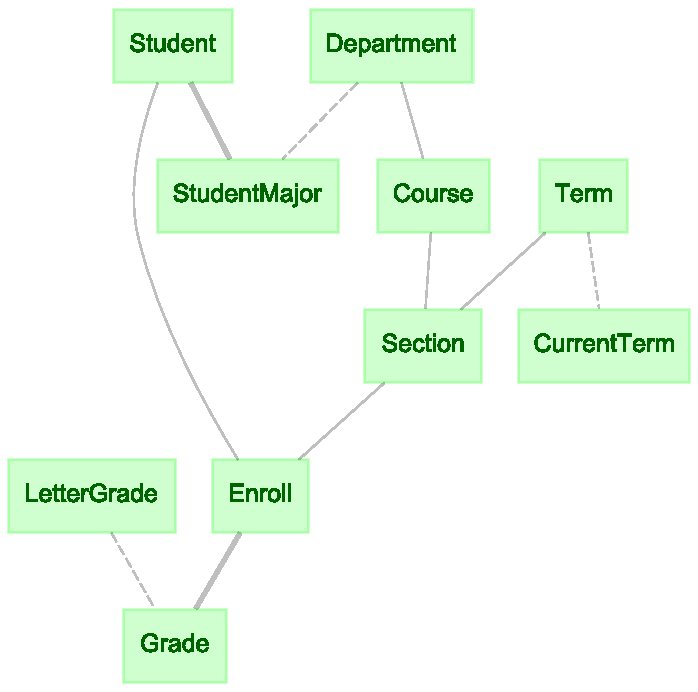
\includegraphics[width=\columnwidth]{uni_erd.pdf}
\caption{The schema diagram of the university database.}
\label{fig:erd}
\end{figure}


\subsubsection{Attributes and their datatypes}
\subsubsection{Primary key}

\subsection{Dependencies}
\subsubsection{Effects of dependencies}
\subsubsection{Primary and secondary dependencies}
\subsubsection{Acyclicity}

\subsection{Schema diagrams}\label{sec:diag}

\section{Data manipulation}\label{sec:manip}
\subsection{Insert}
\subsection{Delete}
\subsection{Cautious update}

\section{Query Expressions}\label{sec:query}
\subsection{Relational operators and expressions}
\subsection{Operational entity integrity}
\subsection{Join compatibility}
\subsection{Restriction}
\subsubsection{Restriction by attribute conditions}
\subsubsection{Restriction by other relations}
\subsubsection{Restriction by a list}

\subsection{Join}
\subsection{Projection}
\subsection{Union}
\subsection{Aggregation}
Aggregation functions cannot be used in restrictions. 
\subsection{Relation U}

\section{Schema Definition --- Advanced.}\label{sec:def2}
\subsection{Dependencies on query expressions}
\subsection{Master-part relationship}
The primary motivation for the master-part relationship is to inform the application that the master and all its parts should always appear together or not at all.  
This usually means using transactions.  
A transaction starts then the master is inserted, then all the parts, and only then the transaction is committed.  
This way all other users only see the master entry when all its parts have been entered.
A part may be in 1-to-1 relationship with its master without any new primary attributes.
\subsection{Dependency properties}

\section{Discussion}
The relational model for databases has been around for nearly fifty years and its use has been standardized by a wide adoption of SQL.
However, some lack of conceptual clarity of SQL and the relational data model make them unwieldy for conceptual design and complex queries. 
As a result, the field has converged on the understanding that database design consists of two distinct components: \emph{conceptual modeling} and \emph{logical modeling} leading to physical implementation. 
Although the Entity Relationship Model was proposed as a model suitable for both conceptual modeling and definition of database schemas, it never replaced the refined data definition languages and evolved into a tool limited to conceptual modeling.  
Furthermore, the ERM's conceptual clarifications chiefly pertain to schema definition and do not provide a data query language with the same level conceptual clarification for derived results as for stored data.

The relational data model and its query languages relational algebra and relational calculus are not concerned with observing. 

SQL in term is implemented to support the general unrefined relational data model while also deviating from it in significant ways. 
Although most SQL programmers 



\appendix

\section{Differences from SQL}
Faithful adherence to the relational data model. 
Native entity integrity.

\subsection{SQL Translations}


\bibliography{DataJoint}

\end{document}
